% Компилира се както с pdfLaTeX, така и с XeLaTeX (напр. в Overleaf)
\documentclass[11pt,a4paper]{article}

\usepackage{iftex}
\ifPDFTeX
  \usepackage[utf8]{inputenc}
  \usepackage[T2A]{fontenc}
  \usepackage[bulgarian]{babel}
\else
  \usepackage{fontspec}
  \setmainfont{DejaVu Serif}
  \setsansfont{DejaVu Sans}
  \setmonofont{DejaVu Sans Mono}
  \usepackage{polyglossia}
  \setdefaultlanguage{bulgarian}
  \setotherlanguage{english}
\fi

\usepackage[margin=1.9cm]{geometry}
\usepackage{tabularx}
\usepackage{graphicx}
\usepackage{float}
\usepackage{caption}
\captionsetup{font=small,labelfont=bf}
\usepackage{booktabs}
\usepackage{enumitem}
\usepackage{titlesec}
\usepackage[hidelinks]{hyperref}

\setlist{nosep,leftmargin=1.4em}
\titlespacing*{\section}{0pt}{1.0ex}{0.6ex}
\titlespacing*{\subsection}{0pt}{0.8ex}{0.4ex}
\setlength{\parskip}{0.2em}
\setlength{\parindent}{0pt}
\emergencystretch=3em
\usepackage{array}
\newcolumntype{L}{>{\raggedright\arraybackslash}X}

\begin{document}

%-------------------------------------------------------------
\begin{center}
  {\Large\bfseries YTKI: Интелигентна мултиагентна система\\[2pt]
  за мониторинг и реакция при инциденти в облачни услуги}\\[6pt]
  {\normalsize Домашна работа 1: описание на темата на курсовата работа}
\end{center}

\begin{center}
\begin{tabular}{ll}
\toprule
\textbf{Име и фамилия} & \textbf{Факултетен номер} \\
\midrule
Йоан Байчев & 0MI0600328 \\
Тугай Кафа & 4MI0600275 \\
Калоян Марков & 4MI0600392 \\
Илиан Запрянов & 8MI0600405 \\
\bottomrule
\end{tabular}
\end{center}

\textbf{Тема:} Интелигентна система за мониторинг, базирана на AI агенти.
Системата работи 24/7 и в реално време приема алерти, логове и health сигнали
от различни landscape-и и среди (dev, staging, int-prod, prod). Тя класифицира
инцидентите и помага на DevOps, SRE и operations екипите да ги разследват и
решават по-бързо.

%-------------------------------------------------------------
\section{Състояние в областта}

Облачните услуги днес рядко са едно приложение. Обикновено става дума за
десетки микроуслуги, пуснати в няколко региона и в отделни среди за
разработка, тестване и продукция. Всяка от тях пише логове, метрики и
трасировки и може да вдигне алерт. Понеже услугите зависят една от друга,
проблем в една централна услуга бързо се отразява и на останалите.
Прекъсванията струват скъпо. Gartner дава ориентировъчна оценка от около
5\,600 долара за минута престой~\cite{gartner}. По данни на Uptime Institute
над 60\% от сериозните прекъсвания през 2022~г. са довели до загуби над
100\,000 долара, а 15\% от тях са надхвърлили 1 милион~\cite{uptime}.

\textbf{Съществуващи инструменти и практики.} За събиране и визуализация на
телеметрия има утвърдени решения като Prometheus, Grafana, Splunk, Datadog и
OpenSearch, а дежурствата обикновено се организират през PagerDuty или
Opsgenie. Подходът Site Reliability Engineering, описан от Google~\cite{sre},
наложи понятия като SLO и error budget, както и т.нар. четири златни сигнала:
latency, traffic, errors и saturation. OpenTelemetry постепенно се превръща в
общ стандарт за събиране на данните.

\textbf{Актуални тенденции.} Gartner въвежда термина AIOps~\cite{aiops} за
използването на машинно обучение в IT операциите: корелация на събития,
откриване на аномалии, търсене на първопричина. С появата на големите езикови
модели (LLM) започнаха да се появяват и агентни системи. В тях няколко
специализирани агента си разпределят разследването (един чете логове, друг
проверява health endpoint-ите, трети гледа зависимостите), а накрая
резултатът се обобщава на разбираем език.

\textbf{Нерешени проблеми.} Инструментите сами по себе си не решават въпроса
какво да се прави с алертите. Първо, те са твърде много и голяма част се
оказват фалшиви или дублирани. Дежурните свикват да ги пренебрегват и
рискуват да пропуснат истински инцидент~\cite{sre}. Второ, данните са
разпръснати в различни системи, а всяка среда се наблюдава поотделно. Трето,
анализът е ръчен: инженерът сам търси логове, проследява зависимости и отваря
тикет, което удължава времето за откриване (MTTD) и за възстановяване (MTTR).
Четвърто, решенията от минали инциденти рядко се записват така, че да могат
да се използват отново. Към това се добавя и регулаторен натиск. Директивата
NIS2~\cite{nis2} задължава операторите на съществени и важни услуги да подават
ранно предупреждение за значим инцидент до 24 часа, така че бързата и
проследима реакция вече е и законово изискване.

%-------------------------------------------------------------
\section{Дефиниране на проблема и обосновка на проекта}

\textbf{Проблем.} Нашият случай е организация, която поддържа облачна
платформа с няколко landscape-а и среди. Само за последните 24 часа в трите
наблюдавани среди (dev, staging и int-prod) са отворени 46 алерта, от които 26
критични, и нито един не е отбелязан като решен. За всеки от тях дежурният
трябва сам да прецени дали е фалшив, дали е локална деградация или реално
прекъсване на услугата, къде е първопричината и чий е компонентът. Това
отнема време, води до грешни ескалации и изтощава хората на смяна. Накрая
рискът се прехвърля към клиентите под формата на нарушени SLA.

\textbf{Предлагано решение.} YTKI е система от AI агенти, която работи
непрекъснато и прекарва всеки входящ алерт през няколко слоя
(фиг.~\ref{fig:architecture}):
\begin{itemize}
  \item \textbf{Ingestion и Broadcasting:} алертите идват през прокси, парсват
  се и се разпращат чрез абонаментен модел към подписчици, които делят общ
  контекст.
  \item \textbf{Planning и Execution:} системата определя какво точно трябва
  да се разследва, разбива го на подзадачи и ги възлага на отделни агенти
  (четене на логове от Cloud Logging, проверка на health endpoint-и, анализ на
  графа на зависимостите).
  \item \textbf{Aggregation и Classification:} резултатите се обединяват и
  инцидентът се класифицира като фалшив алерт, деградация или прекъсване, с
  вероятност за всяка категория. При нужда се пускат Playwright сценарии или
  автоматизирани потоци в n8n.
  \item \textbf{Operation:} чрез мапинг се намира отговорният компонент,
  създава се събитие в Splunk и се отваря тикет.
  \item \textbf{Learning:} историята на инцидентите се пази и върху нея се
  обучават класически модели (логистична регресия, random forest), за да
  става класификацията по-точна с времето.
\end{itemize}

\begin{figure}[H]
  \centering
  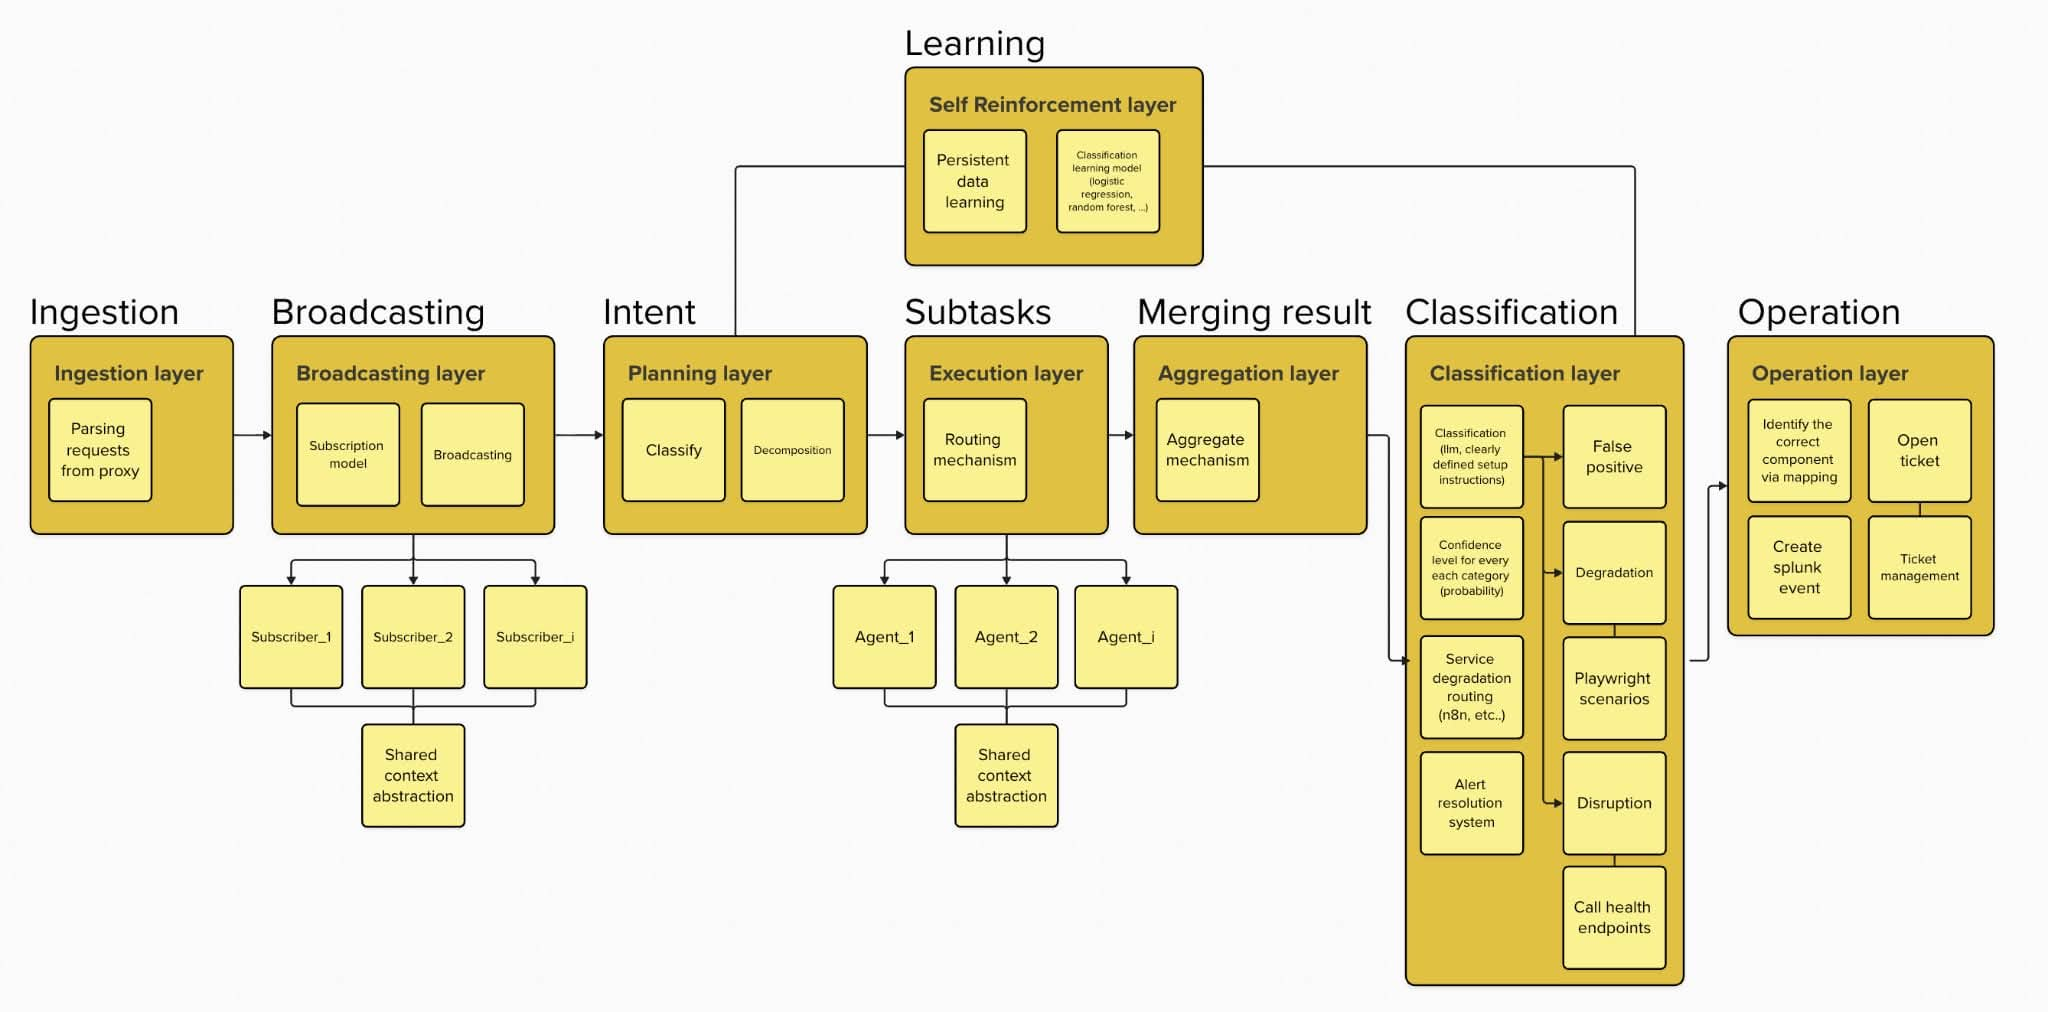
\includegraphics[width=0.92\textwidth]{architecture.jpeg}
  \caption{Архитектура на YTKI: от приемането на алерта до оперативното
  действие, с обратна връзка към слоя за самообучение.}
  \label{fig:architecture}
\end{figure}

Част от системата вече съществува като работещ прототип: табло с обобщение по
среди, златни сигнали, граф на зависимостите между услугите, оценка на
каскадния риск и хипотези за първопричина. Има и чат („Ask Alerts“), в който
инженерът пита на свободен език какво се случва с дадена услуга, а системата
сама изтегля и анализира логовете.

\textbf{Обосновка.} Основната полза е във времето. Когато дежурният получи
алерта заедно с готов анализ (логове, засегнати услуги, вероятна причина), той
не започва от нулата и инцидентът се решава по-бързо. Отсяването на фалшивите
алерти намалява шума и умората на екипа, а единният изглед спестява
превключването между инструменти и среди. С натрупването на история
системата класифицира все по-точно. Бързото откриване и документиране на
инцидентите помага на организацията и да спазва сроковете по NIS2. За
крайните клиенти ползата е пряка: по-редки и по-кратки прекъсвания.

%-------------------------------------------------------------
\section{Заинтересовани лица}

\small
\begin{tabularx}{\textwidth}{@{}>{\raggedright\arraybackslash}p{3.2cm}p{2.1cm}LL@{}}
\toprule
\textbf{Заинтересовано лице} & \textbf{Вид} & \textbf{Нужди} & \textbf{Роля в проекта} \\
\midrule
DevOps и SRE инженери, дежурни (on-call) & Вътрешни &
По-малко шум, бърз анализ на първопричината, един изглед за всички среди &
Основни потребители; задават изискванията, тестват системата и дават обратна връзка \\
\addlinespace[2pt]
Разработчици и собственици на услуги & Вътрешни &
Да знаят кой компонент е засегнат и защо; тикети с готов контекст &
Поддържат мапинга на компонентите, health endpoint-ите и правилата за алерти; получават ескалациите \\
\addlinespace[2pt]
Ръководство (engineering managers, product owners) & Вътрешни &
Видимост върху надеждността, спазване на SLA, по-ниски оперативни разходи &
Спонсори; осигуряват ресурси и определят приоритета на внедряването \\
\addlinespace[2pt]
Екипи по сигурност и съответствие & Вътрешни &
Проследимост на инцидентите и навременно докладване &
Поставят изисквания за одит, защита на данните и достъп до логове \\
\addlinespace[2pt]
Проектният екип (авторите) & Вътрешни &
Реални данни и достъп до средите за разработка &
Проектират, разработват и поддържат системата \\
\addlinespace[2pt]
Клиенти (тенанти) на облачните услуги & Външни &
Висока наличност, бързо възстановяване, ясна комуникация при проблем &
Косвени бенефициенти; по техните инциденти и обратна връзка се оценява ефектът \\
\addlinespace[2pt]
Доставчици на платформи и инструменти (облак, логване, Splunk, LLM) & Външни &
Коректна интеграция и използване на API-тата им &
Осигуряват инфраструктурата и източниците на данни, от които системата зависи \\
\addlinespace[2pt]
Регулаторни органи (по NIS2) & Външни &
Навременно и пълно докладване на значими инциденти &
Определят нормативната рамка, на която системата трябва да отговаря \\
\bottomrule
\end{tabularx}
\normalsize

%-------------------------------------------------------------
\begin{thebibliography}{9}\footnotesize
\setlength{\itemsep}{0pt}
\bibitem{gartner} A. Lerner, \emph{The Cost of Downtime}, Gartner Blog, 2014.
\bibitem{uptime} Uptime Institute, \emph{Annual Outage Analysis 2022}, Uptime Institute, 2022.
\bibitem{sre} B. Beyer, C. Jones, J. Petoff, N. R. Murphy, \emph{Site Reliability Engineering: How Google Runs Production Systems}, O'Reilly, 2016.
\bibitem{aiops} Gartner, \emph{Market Guide for AIOps Platforms}, Gartner Research, 2017.
\bibitem{nis2} Директива (ЕС) 2022/2555 на Европейския парламент и на Съвета относно мерки за високо общо ниво на киберсигурност в Съюза (NIS2), ОВ L 333, 27.12.2022.
\end{thebibliography}

\end{document}
